\section{The problem statement}

This document contains the solution for the surface code quantum error correction problem. Sergei's
questions are rendered in \begin{\QuestionColor}\QuestionColorName\ color\end{\QuestionColor}. The
project repository is hosted on
Github\footnote{Github repo: \url{https://github.com/sergei-mironov/qecsurface}}.

\vsp

Your task is to \textbf{set up a distance 3 surface code using PennyLane}. If you are not familiar
with Surface Codes, this may be a very useful resource: \url{https://arxiv.org/pdf/1404.3747}. Try
to simulate \textbf{at least one cycle of the quantum error correction scheme} and give a quick
interpretation of the results. Try \textbf{adding some noise to the circuit} (for example, add a
random bit-flip in the circuit), and see what happens to the measurement. You should
\textbf{describe in words how the decoding would happen}. If you have the extra time, feel free to
also implement some \textbf{simple decoding protocols}. The expected output of this exercise is a
Jupyter Notebook. But feel free to deliver your answer in whichever medium you see fit. Most
importantly, try to learn about quantum error correction and give us an insight into the way you
tackle difficult, unseen problems.


\section{Literature overview}

\ls \tcite{Tomita2014}. References:
    \ls \t{[2]} \tcite{Brun2020}
    \li \t{[6]} \u{Surface codes: Towards practical large-scale quantum computation}{https://arxiv.org/pdf/1208.0928}
        by Austin G. Fowler (2012)
    \le
\li \u{Wiki about the Shor code}{https://en.wikipedia.org/wiki/Quantum_error_correction\#Shor_code}
\li IQC 2024 Lecture 29 \u{Quantum Error Correction: Surface Codes}{https://opencourse.inf.ed.ac.uk/sites/default/files/https/opencourse.inf.ed.ac.uk/iqc/2024/iqclecture29_0.pdf}
\li Coursera course Hands-on quantum error correction
    \ls \href{https://journals.aps.org/prx/pdf/10.1103/PhysRevX.2.041003}{Topological Code Autotune}
        by Austin G. Fowler (2012)
    \le
\li \href{https://arxiv.org/abs/2307.14989}{Decoding algorithms for surface codes} by lOlius (2024)
    \ls \t{50} \href{https://arxiv.org/abs/2112.03708}{Realizing Repeated Quantum Error Correction in a Distance-Three Surface Code}
    \li \t{51} \u{Suppressing quantum errors by scaling a surface code logical qubit}{https://arxiv.org/abs/2207.06431}
    \le
\li \tcite{Nielsen2010}
\le


\section{Some theory}

In this section, we summarize our current understanding of the problem domain.

\subsubsection*{Quantum error correction codes}

Quantum error correction codes (QECC) are techniques used to protect quantum information from errors
due to decoherence, noise, and other quantum imperfections. They work by encoding logical quantum
bits (qubits) into a larger number of physical qubits, allowing for the detection and correction of
errors that can occur during quantum computation or storage.

\subsubsection*{Common error correction codes}

\begin{enumerate}
  \item \textbf{Bit-flip code:} One of the simplest quantum error correction codes, the bit-flip
  code protects against bit-flip errors by encoding each logical qubit using three physical qubits.

  \item \textbf{Phase-flip code:} Similar to the bit-flip code, the phase-flip code protects against
  phase-flip errors by encoding each logical qubit using three physical qubits.

  \item \textbf{Shor code:} The Shor code is a 9-qubit code that can protect against both bit-flip
  and phase-flip errors, essentially combining the bit-flip and phase-flip codes.

  \item \textbf{Steane code:} The Steane code is a 7-qubit code that can correct arbitrary
  single-qubit errors. It is based on classical error-correcting codes and is more efficient than
  the Shor code.

  \item \textbf{Five-qubit code:} Also known as the perfect code, this is the smallest possible code
  that can correct arbitrary single-qubit errors, using just five physical qubits to encode one
  logical qubit.

  \item \textbf{Surface codes:} Surface codes are defined on a lattice and are known for their high
  threshold for error tolerance and efficient implementation.
\end{enumerate}


\subsubsection*{Code space}

\textit{Code space} refers to the subspace of a quantum Hilbert space in which the logical qubits
are encoded.

We assume that every practical QECC has a code space large enough to encode at least one qubit, that
is, the $\Hilb{1}$.

\vsp

For example, the code space of the Stean code is spanned across the following vectors

\[
\ket{0_L} = \frac{1}{\sqrt{8}} \left( \ket{0000000} + \ket{1010101} + \ket{0110011} + \ket{1100110}
+ \ket{0001111} + \ket{1011010} + \ket{0111100} + \ket{1101001} \right)
\]

\vsp

\[
\ket{1_L} = \frac{1}{\sqrt{8}} \left( \ket{1111111} + \ket{0101010} + \ket{1001100} + \ket{0011001}
+ \ket{1110000} + \ket{0100101} + \ket{1000011} + \ket{0010110} \right)
\]


\subsubsection*{Stabilizer codes}

The stabilizer formalism is a framework used in quantum error correction to describe quantum states
and codes. It is based on the concept of stabilizer groups, which are sets of commuting operators
from the Pauli group that stabilize (or leave unchanged) a particular subspace of a quantum system's
Hilbert space, known as the code space.

\vsp

In the context of a quantum error-correcting code (QECC), stabilizer formalism describes logical
states such as \(\ket{0_L}\) and \(\ket{1_L}\) of a QECC by specifying the stabilizers that leave
these states unchanged.  These logical states are defined as the common +1 eigenstates of the
stabilizer generators.

\vsp

The \textbf{Stabilizer Theorem} provides an important property that helps define valid stabilizer
codes: A valid stabilizer code must have a stabilizer group composed of operators that do not
include the negative identity operator \(-I\) as an element.

\begin{itemize}
  \item Every element of the stabilizer group must be a Hermitian operator with eigenvalues \( \pm 1
\). The presence of \(-I\) would imply that the eigenvalue \(-1\) is always included, which
conflicts with the requirement that the identity operator \(I\) (with eigenvalue \(+1\)) must be an
element of the group.
  \item The requirement to exclude \(-I\) ensures the stabilizer group forms a valid subgroup of the
Pauli group, allowing the stabilizer code to properly define the code space and detect/correct
errors without inherent contradictions.
\end{itemize}

\subsection{Setup}

The project could be cloned from the GitHub repository
\url{https://github.com/sergei-mironov/qecsurface}. The repository contains sourceable file
\t{env.sh} which adjusts \t{PATH} and \t{PYTHONPATH} environment variables to make project specific
shell-scripts and Python modules available.

Overall, the typical initizlization command sequence is follows:

\begin{sh}
$ git clone https://github.com/sergei-mironov/qecsurface
$ cd qecsurface
$ . env.sh
$ ipython # Enter IPython interactive shell
>>> from quecsurface import *
>>> from quecsurface_tests import *
\end{sh}

\begin{comment}
\begin{python}
import matplotlib.pyplot as plt
from qecsurface import *
\end{python}
\begin{result}
\end{result}
\end{comment}

\subsection{Overview}

The qecsurface project defines the following main Python modules:

\ls \t{qecsurface.type} defines a minimalistic domain-specific language for quantum circuits
    modeling. The main data structure for circuits is named $FTCircuit$ where FT stands for
    "Fault Tolerant".
\li \t{qecsurface.pennylane} defines routines which lower $FTCircuits$ to PennyLane circuits.
\li Finally, \t{qecsurface.qeccs} introduces $FTCircuit \to FTCircuit$ mappings
    which implement various Quantum error correction schemes.
\le

\subsection{Base Types}

\subsubsection{Quantum Operations}

  \begin{comment}
    \begin{sh}
    printf '\\begin{%s}\n' 'python'
    cat $PROJECT_ROOT/python/qecsurface/type.py | sedlines.sh 'Quantum operation definitions'
    printf '\\end{%s}\n' 'python'
    \end{sh}
  \end{comment}

  %result
  \begin{python}
  class OpName(Enum):
    """ Quantum operation labels """
    I = 0
    X = 1
    Z = 2
    H = 3

  def opname2str(n:OpName)->str:
    return {OpName.I:'I', OpName.H:'H', OpName.Z:'Z', OpName.X:'X'}[n]

  # Common type alias for quantum operations
  type FTOp[Q] = Union["FTInit[Q]", "FTPrim[Q]", "FTCond[Q]", "FTCtrl[Q]", "FTMeasure[Q]",
                       "FTErr[Q]"]

  @dataclass
  class FTInit[Q]:
    """ Primitive quantum operation acting on one qubit. """
    qubit:Q
    alpha:complex
    beta:complex

  @dataclass
  class FTPrim[Q]:
    """ Primitive quantum operation acting on one qubit. """
    name:OpName
    qubits:list[Q]

  @dataclass
  class FTCtrl[Q]:
    """ Quantum control operation acting on two qubits. """
    control:Q
    op:FTOp[Q]

  # Syndrome test measurement label encodes a layer, the syndrome type and the qubit labels
  type MeasureLabel[Q] = tuple[int,OpName,tuple[Q,...]]

  @dataclass
  class FTMeasure[Q]:
    """ Quantum measure oprtation which acts on a `qubit`. Measurement result is assiciated with a
    `label`. """
    qubit:Q
    label:MeasureLabel[Q]

  @dataclass
  class FTCond[Q]:
    """ A quantum operation applied if a classical condition is met. """
    cond:Callable[[dict[MeasureLabel[Q],int]],bool]
    op:FTOp[Q]

  @dataclass
  class FTErr[Q]:
    """ Apply an error to `phys` physical qubit constituting the logical qubit Q. """
    qubit:Q
    phys:int
    name:OpName
  \end{python}
  %noresult

\subsubsection{Quantum circuits}

  \begin{comment}
    \begin{sh}
    printf '\\begin{%s}\n' 'python'
    cat $PROJECT_ROOT/python/qecsurface/type.py | sedlines.sh 'Quantum circuit definitions'
    printf '\\end{%s}\n' 'python'
    \end{sh}
  \end{comment}

  %result
  \begin{python}
  # Common type alias for quantum circuits, where Q is type of qubit label.
  type FTCircuit[Q] = Union["FTOps[Q]", "FTComp[Q]"]

  @dataclass
  class FTOps[Q]:
    """ A primitive circuit consisting of a tape of operations. """
    ops:list[FTOp[Q]]

  @dataclass
  class FTComp[Q]:
    """ Composition of circuits, also known as circuit tensor product. """
    a: FTCircuit[Q]
    b: FTCircuit[Q]
  \end{python}
  %noresult


\subsubsection{Mapping form circuit to circuit}

The map operation is defined on $FTCircuit_q$ is

$$
\forall a,b \suchthat map\_circuit : Map_{a,b} \to FTCircuit_a \to FTCircuit_b
$$

The subsequent quantum error correction algorithms are defined as derived classes of the
$Map_{a,b}$ base class.

  \begin{comment}
    \begin{sh}
    printf '\\begin{%s}\n' 'python'
    cat $PROJECT_ROOT/python/qecsurface/type.py | sedlines.sh 'Circuit mapping'
    printf '\\end{%s}\n' 'python'
    \end{sh}
  \end{comment}

  %result
  \begin{python}
  @dataclass
  class Map[Q1,Q2]:
    """ Base class for stateful circuit mapping algorithms. """
    def map_op(self, op:FTOp[Q1]) -> FTCircuit[Q2]:
      """ Maps an operation of a source circuit into a destination circuit. """
      raise NotImplementedError


  def map_circuit[Q1,Q2](c:FTCircuit[Q1], m:Map[Q1,Q2]) -> FTCircuit[Q2]:
    """ Maps the circuit `c` by mapping each its operation and taking a compostion """
    def _traverse_op(op:FTOp[Q1], acc) -> None:
      return FTComp(acc, m.map_op(op))
    return traverse_circuit(c, _traverse_op, FTOps([]))
  \end{python}
  %noresult

\subsubsection{Example: Quantum teleportation}

  \begin{python}
  circuit_ft = FTComp(
    FTOps([
      FTInit(qubit=0, alpha=1.0, beta=0.0),         # Initialize the qubit in a known state
      FTPrim(OpName.H, [1]),                        # Apply Hadamard to qubit 1
      FTCtrl(control=1, op=FTPrim(OpName.X, [2])),  # Entangle qubits 1 and 2
      FTCtrl(control=0, op=FTPrim(OpName.X, [1])),  # Bell state preparation
      FTPrim(OpName.H, [0]),                        # Apply Hadamard to qubit 1
      FTMeasure(qubit=0, label="mZ"),
      FTMeasure(qubit=1, label="mX")
    ]),
    FTComp(
      FTOps([
        FTCond(lambda m: m["mX"] == 1, FTPrim(OpName.X, [2]))  # Conditional X based on m0
      ]),
      FTOps([
        FTCond(lambda m: m["mZ"] == 1, FTPrim(OpName.Z, [2]))  # Conditional Z based on m1
      ])
    )
  )
  cPL = to_pennylane_mcm(circuit_ft)
  qml.draw_mpl(cPL)()
  plt.savefig('../img/teleport.png')
  \end{python}

  \begin{comment}
  \begin{result}
  \end{result}
  \end{comment}

\begin{figure}[h!]
  \centering
  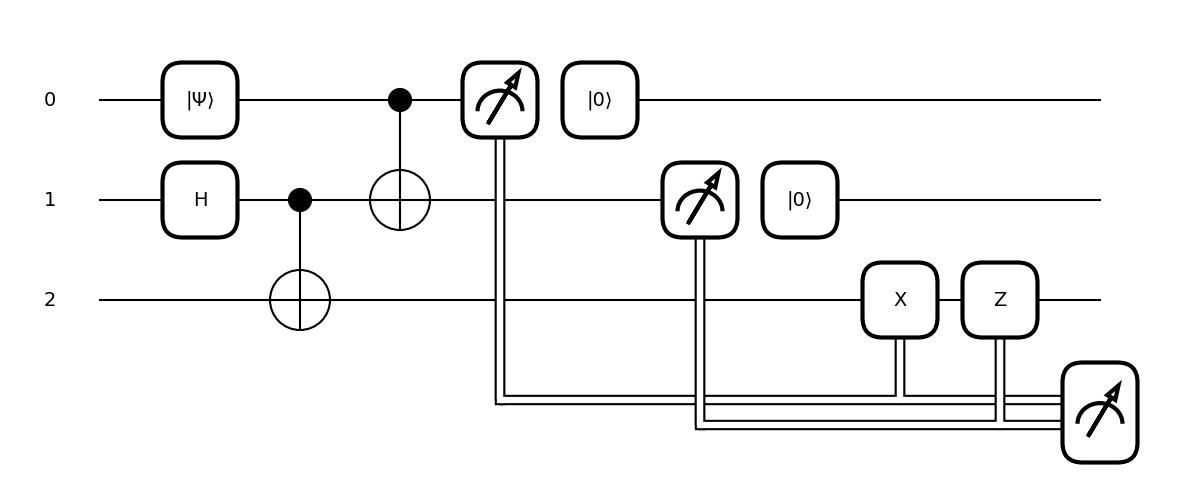
\includegraphics[width=0.5\textwidth]{../img/teleport.png}
  \caption{Quantum teleportation circuit.}
  \label{fig:teleport}
\end{figure}


\subsubsection{Example: Bitflip code}

  \begin{comment}
    \begin{sh}
    printf '\\begin{%s}\n' 'python'
    cat $PROJECT_ROOT/python/qecsurface/qeccs.py | \
      sedlines.sh 'Bitflip' | \
      sed '/^    /,/^$/d' | sed 's/:$//'
    printf '\\end{%s}\n' 'python'
    \end{sh}
  \end{comment}

  %result
  \begin{python}
  @dataclass
  class Bitflip[Q1,Q2](Map[Q1,Q2])
    """ Maps quantum circuit into a quantum circuit with Bitflip quantum error correction. """
    qmap:dict[Q1,tuple[list[Q2],list[Q2]]]
    layer:int = 0

    def _next_layer(self) -> int
    def _error_correction_cycle(self, q:Q1) -> FTCircuit[Q2]
    def map_op(self, op:FTOp[Q1]) -> FTCircuit[Q2]
  \end{python}
  %noresult

\subsection{Quantum Error Correction with Surface25u}

\subsubsection{Overview}

We implement the Surface25 (unified) quantum error correction code following \cite{Tomita2014}.  We
consider syndrome qubits ideal so we unify them as a single model qubit to speed up the
computations.

\begin{figure}[h!]
  \centering
  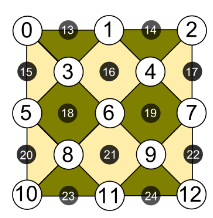
\includegraphics[width=0.2\textwidth]{../img/surface25.png}
  \caption{Surface 25 quantum error correction code.}
  \label{fig:surface25}
\end{figure}


\subsubsection{Hadamard tests}

The backbone of the suface quantum error correction codes are Hadamard tests projecting the quantum
state to one of stabilizer eigenstates and revealing its signs. We define these tests as follows:

  \begin{comment}
    \begin{sh}
    printf '\\begin{%s}\n' 'python'
    cat $PROJECT_ROOT/python/qecsurface/qeccs.py | \
      sedlines.sh 'Stabilizer tests'
    printf '\\end{%s}\n' 'python'
    \end{sh}
  \end{comment}

  %result
  \begin{python}
  def stabilizer_test_X[Q](tile:FTPrim[Q], syndrome:Q, ml:MeasureLabel[Q]) -> FTCircuit[Q]:
    """ Define a stabilizer X-test circuit. """
    assert tile.name == OpName.X, tile
    return FTOps([
      FTPrim(OpName.H, [syndrome]),
      *[FTCtrl(control=syndrome, op=FTPrim(OpName.X, [qubit_label]))
        for qubit_label in tile.qubits
      ],
      FTPrim(OpName.H, [syndrome]),
      FTMeasure(qubit=syndrome, label=ml)
    ])

  def stabilizer_test_Z[Q](tile:FTPrim[Q], syndrome:Q, ml:MeasureLabel[Q]) -> FTCircuit[Q]:
    """ Define a stabilizer Z-test circuit. """
    assert tile.name == OpName.Z, tile
    return FTOps([
      *[FTCtrl(control=qubit_label, op=FTPrim(OpName.X, [syndrome]))
        for qubit_label in tile.qubits
      ],
      FTMeasure(qubit=syndrome, label=ml)
    ])
  \end{python}
  %noresult


  \begin{comment}
  \begin{python}
  cPL = to_pennylane_mcm(stabilizer_test_X(FTPrim(OpName.X, [0,1,2]), 3, None))
  qml.draw_mpl(cPL)()
  plt.savefig('../img/stabilizer_test_X.png')
  cPL = to_pennylane_mcm(stabilizer_test_Z(FTPrim(OpName.Z, [0,1,2]), 3, None))
  qml.draw_mpl(cPL)()
  plt.savefig('../img/stabilizer_test_Z.png')
  \end{python}

  \begin{result}
  \end{result}
  \end{comment}

\begin{figure}[h!]
  \centering
  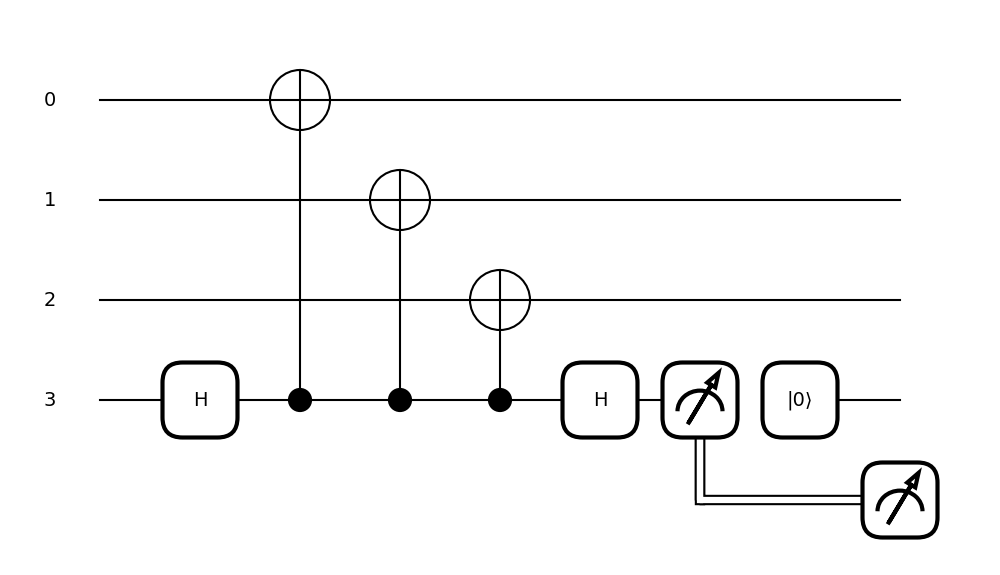
\includegraphics[width=0.4\textwidth]{../img/stabilizer_test_X.png}
  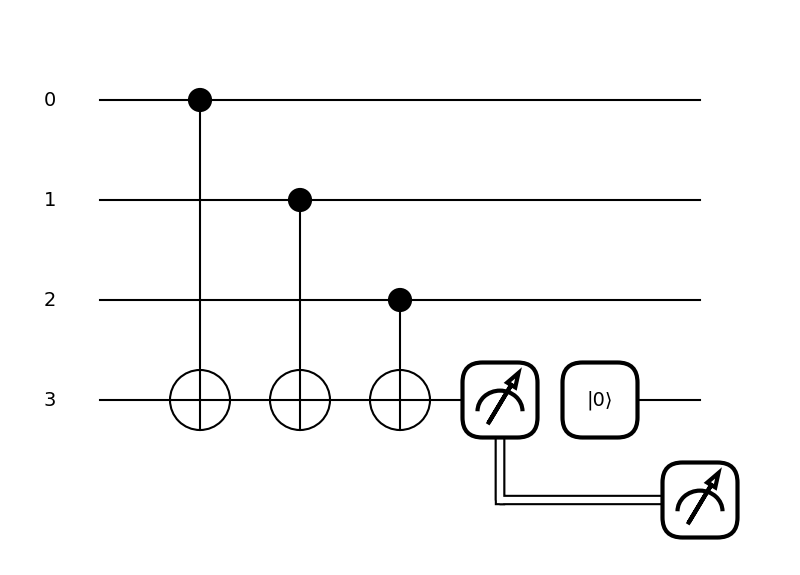
\includegraphics[width=0.4\textwidth]{../img/stabilizer_test_Z.png}
  \caption{Stabilizer X-test and stabilizer Z-test.}
\end{figure}

\subsubsection{Error correction code primitives}

We split the implementation in several functions:

\ls The Surface25 stabilizer layout is defined as a constant:

  \begin{comment}
    \begin{sh}
    printf '\\begin{%s}\n' 'python'
    cat $PROJECT_ROOT/python/qecsurface/qeccs.py | \
      sedlines.sh 'surface25_stabilizers'
    printf '\\end{%s}\n' 'python'
    \end{sh}
  \end{comment}

  %result
  \begin{python}
  def surface25_stabilizers() -> list[FTPrim[int]]:
    """ Surface25 stabilizers. Qubit labels may be interpreted as indices. """
    def X(data):
      return FTPrim(OpName.X, data)
    def Z(data):
      return FTPrim(OpName.Z, data)
    return [
              X([0,1,3]), X([1,2,4]),
      Z([0,3,5]), Z([1,3,4,6]), Z([2,4,7]),
             X([3,5,6,8]), X([4,6,7,9]),
      Z([5,8,10]), Z([6,8,9,11]), Z([7,9,12]),
             X([8,10,11]), X([9,11,12]),
    ]
  \end{python}
  %noresult


\li The detector function converts the stabilizer layout into a sequence of Hadamard tests and
    returns syndrome measurement labels along with the resulting circuit.

  \begin{comment}
    \begin{sh}
    printf '\\begin{%s}\n' 'python'
    cat $PROJECT_ROOT/python/qecsurface/qeccs.py | \
      sedlines.sh 'surface25u_detect'
    printf '\\end{%s}\n' 'python'
    \end{sh}
  \end{comment}

  %result
  \begin{python}
  def surface25u_detect[Q](
    data: list[Q], syndromes: list[Q], layer:int=0
  ) -> tuple[FTCircuit[Q],list[MeasureLabel]]:
    """ Build the surface25u error detection circuit. Return the circuit alongside with a list of
    mid-circuit measurement labels. """
    assert len(data) == 13, f"Expected 13 data qubit labels, got {data}"
    assert len(syndromes) == 1, f"Expected 1 syndrome qubit label, got {syndrome}"
    syndrome = syndromes[0]
    labels = []

    def _to_hadamard_test(op):
      qubits = [data[q] for q in op.qubits]
      labels.append((layer,op.name,tuple(qubits)))
      if op.name == OpName.X:
        return stabilizer_test_X(FTPrim(OpName.X, qubits), syndrome, labels[-1])
      elif op.name == OpName.Z:
        return stabilizer_test_Z(FTPrim(OpName.Z, qubits), syndrome, labels[-1])
      else:
        raise ValueError(f"Unrecognized op {op}")

    return reduce(FTComp, map(_to_hadamard_test, surface25_stabilizers())), labels
  \end{python}
  %noresult

\li The correction implements a simple decoding protocol to fix any single-qubit errors.

  \begin{comment}
    \begin{sh}
    printf '\\begin{%s}\n' 'python'
    cat $PROJECT_ROOT/python/qecsurface/qeccs.py | \
    sedlines.sh 'surface25u_correct'
    printf '\\end{%s}\n' 'python'
    \end{sh}
  \end{comment}

  %result
  \begin{python}
  def surface25u_correct[Q](data:list[Q], layer0:int, layer:int) -> FTCircuit[Q]:
    """ Build the surface25u error correction circuit assuming `layer` measurememnts are available.
    Use `layer0` measurements as a reference. """
    def _corrector(op, opc, d):
      def _cond(msms):
        neigb = [l[2] for l in list(msms.keys()) if l[0]==layer and l[1]==op and (d in l[2])]
        others = [l[2] for l in list(msms.keys()) if l[0]==layer and l[1]==op and (d not in l[2])]
        return reduce(
          lambda a,b: a & b, [
            *[(msms[(layer0,op,n)] != msms[(layer,op,n)]) for n in neigb],
            *[(msms[(layer0,op,n)] == msms[(layer,op,n)]) for n in others],
          ]
        )
      return FTCond(_cond, FTPrim(opc,[d]))
    return FTComp(
      FTOps([_corrector(OpName.X, OpName.Z, d) for d in data]),
      FTOps([_corrector(OpName.Z, OpName.X, d) for d in data])
    )
  \end{python}
  %noresult

\li In addition, we define an utility syndrome printing function

  \begin{comment}
    \begin{sh}
    printf '\\begin{%s}\n' 'python'
    cat $PROJECT_ROOT/python/qecsurface/qeccs.py | \
    sedlines.sh -C 'surface25u_print2' | head -n 1
    printf '\\end{%s}\n' 'python'
    \end{sh}
  \end{comment}

  %result
  \begin{python}
  def surface25u_print2(msms:dict[MeasureLabel,int], flt:list[MeasureLabel], ref_layer:int=0)
  \end{python}
  %noresult

\le

\subsubsection{Example: full error correction cycle}

We demonstrate the usage with the following code. First, we initialize the $\ket{0_L}$ state by
passing the $\ket{0}$ through the detection circuit and measuring stabilizer signs. Next, we
introduce an error on the sixth qubit. Finally, we apply the error correction cycle where we use the
stabilizer signs obtained initially.

  \begin{python}
  data, syndrome = list(range(13)), [13]
  layer0, layer1, layer2 = 0, 1, 2
  init, ml1 = surface25u_detect(data, syndrome, layer0)
  err = FTOps([FTPrim(OpName.X,[6]),
               FTPrim(OpName.Z,[6])])
  detect, ml2 = surface25u_detect(data, syndrome, layer1)
  correct = surface25u_correct(data, layer0, layer1)
  cPL = to_pennylane_mcm(reduce(FTComp, [init, err, detect, correct]))
  msms = cPL()
  print(surface25u_print2(msms, ml2))
  \end{python}

We visuzlize the error syndrome before the correction.

  \begin{result}

  o   o   o
    o Z o 
  o X o X o
    o Z o 
  o   o   o

  \end{result}

We make sure the error is gone by applying the final detection and re-running the simulation.

  \begin{python}
  check, ml3 = surface25u_detect(data, syndrome, layer2)
  cPL = to_pennylane_mcm(reduce(FTComp, [init, err, detect, correct, check]))
  msms = cPL()
  print(surface25u_print2(msms, ml3))
  \end{python}

  \begin{result}

  o   o   o
    o   o 
  o   o   o
    o   o 
  o   o   o

  \end{result}

\subsubsection{High-level interface: circuit mapper}

Finally, we wrap these functions into the \t{Surface25u} circuit mapper interface.

  \begin{comment}
    \begin{sh}
    printf '\\begin{%s}\n' 'python'
    cat $PROJECT_ROOT/python/qecsurface/qeccs.py | \
    sedlines.sh -C --filter 4 'Surface25u'
    printf '\\end{%s}\n' 'python'
    \end{sh}
  \end{comment}

  %result
  \begin{python}
  @dataclass
  class Surface25u[Q1, Q2](Map[Q1, Q2])
    qmap: dict[Q1, tuple[list[Q2], Q2]]
    _layer: int = 0
    _layers0: dict[Q1, int] = field(default_factory=dict)
    _mls: dict[Q1, list[MeasureLabel]] = field(default_factory=lambda: defaultdict(list))

    def _next_layer(self) -> int
    def _error_correction_cycle(self, q:Q1, layer0:int) -> FTCircuit[Q2]
    def map_op(self, op: FTOp[Q1]) -> FTCircuit[Q2]
  \end{python}
  %noresult

\section{Questions}


\subsection{Logical state initialization}

\begin{QUESTION}
One thing that is not very clear to me is: what overall usage scheme should I aim for? I saw two
candidates.

\ls Receive a 1-qubit quantum state $\ket{\psi} = \alpha\ket{0} + \beta\ket{1}$ as input. Encode it
    using QECC into the superposition of logical states $\ket{\psi_L} = \alpha\ket{0_L} +
    \beta\ket{1_L}$. Pass it through a noisy quantum channel and decode it back into the original
    $\ket{\psi}$.
\li Initialize the logical qubit with the logical zero state $\ket{0_L}$. Apply logical operations
    such as $X_L$, $Z_L$, or others (TODO: specify which ones exactly) to perform fault-tolerant
    computations, e.g., obtain a desired $\ket{\psi_L}$. Measure it and interpret the results in an
    algorithm-specific way.
\le
\end{QUESTION}

\subsection{Access to mid-circuit measurements in PennyLane}

\begin{QUESTION}
Is it possible to get a direct access to mid-circuit measurements in PennyLane during the
simulation?
\end{QUESTION}

\vsp

As of the time of writing, it appears that PennyLane cannot provide immediate measurement results
prior to the conclusion of a simulation. Instead, it offers a \t{MeasurementResult} promise, which
only supports basic operations. See
\u{Documentation link}{https://docs.pennylane.ai/en/stable/code/api/pennylane.measure.html}.

% \input{_discussions.tex}

